% !TeX root = ../main.tex

\section{1D Digital filters}
\begin{center}
    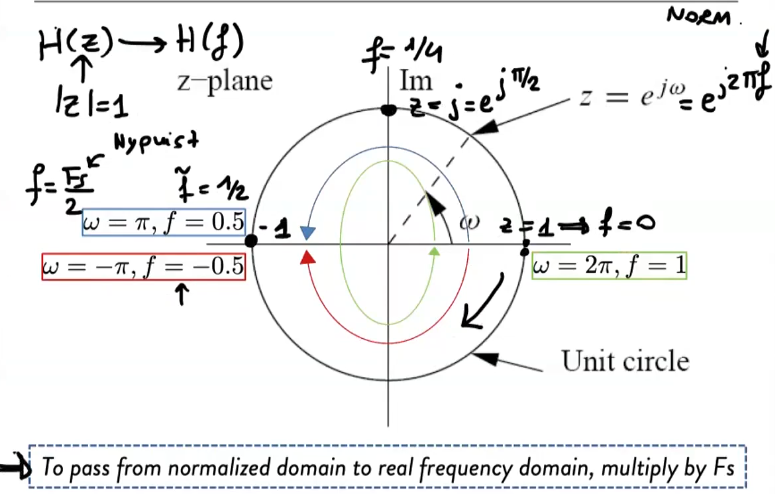
\includegraphics[width=1\textwidth]{images/zero_pole.png}
\end{center}
If asks for $Hz$ domain, multiply by $F_s$. Reminder, a filter:
\begin{LARGE}    
    $$
    H(z)=\frac{
        \sum_{k=0}^Nb_kz^{-k}
    }{\sum_{k=0}^Da_kz^{-k}}=
    z^{D-N}\frac{b_0}{a_0}\frac{
        \prod_{i=1}^N(z-z_i)
    }{\prod_{i=1}^N(z-p_i)}=
    \frac{b_0}{a_0}\frac{
        \prod_{i=1}^N(1-z_iz^{-1})
    }{\prod_{i=1}^N(1-p_iz^{-1})}
    $$
\end{LARGE}
\begin{itemize}
    \item The poles
    \begin{itemize}
        \item Are associated with the autoregressive part, they generate IIR filter $z\rightarrow p_i$, in the frequency the filter will increase $H(f)$
        \item The filter amplitude response enhances frequencies which are near the poles
        \item If poles are outside the unit circle and the filter is causal, the system is unstable
    \end{itemize}
    \item The zeros
    \begin{itemize}
        \item Are associated with the moving average of the filter, they generate FIR filters
        \item The filter amplitude response attenuates frequencies which are near the zero
        \item Zeros influence also the phase of the filter (they do not influence stability)
        \begin{itemize}
            \item Minimum phase zeros if $z<1$, inside unit circle
            \item Maximum phase zeros if $z\geq 1$, outside unit circle
        \end{itemize}
    \end{itemize}
\end{itemize}

\subsection{Filter design: remarkable LTI filters}
\begin{itemize}
    \item Place poles close tot he unit circle in frequencies that must be emphasized
    \item Place zeros according to the desired phase response, the closer are to the unit circle the higher frequency attenuation
\end{itemize}

\subsubsection{Notch}
I want to delete a specific frequency:
\begin{enumerate}
    \item Put two complex zeros on the unit circle
    \item Put two poles with absolute value less than 1, close to unit circle
\end{enumerate}
\begin{center}
    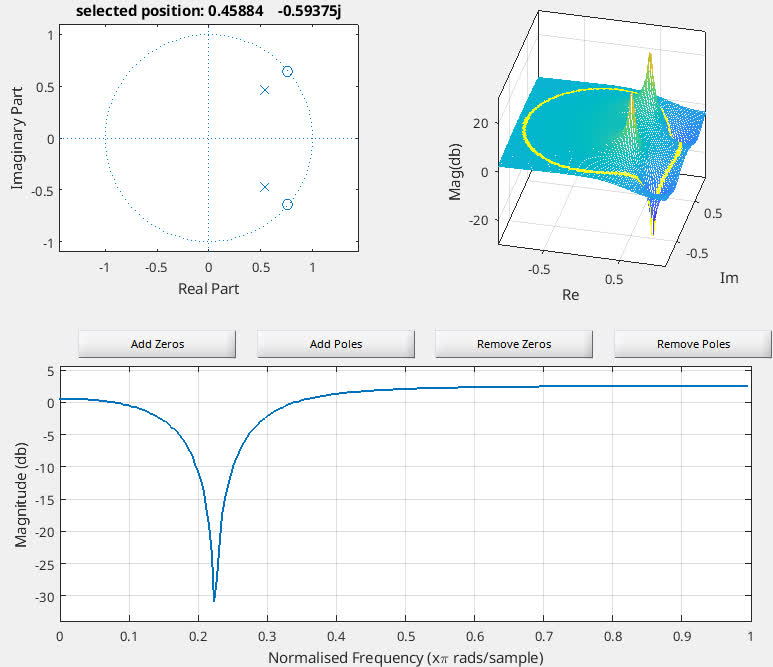
\includegraphics[width=1\textwidth]{images/notch.png}
\end{center}

\subsubsection{Magnitude square function}
The magnitude response of a LTI system is:
$$
M(f)=|H(f)|^2=H(f)\cdot H^*(f)=H(z)\cdot H^*(z^{-1})\big|_{|z|=1}
$$
Given a generic rational transfer function
$$
H(z)=\frac{b_0}{a_0}\frac{
    \prod_{i=1}^N(1-z_iz^{-1})
}{\prod_{i=1}^N(1-p_iz^{-1})}
$$
$$
\Downarrow
$$
$$
M(z)=H(z)H^*(z^{-1})=\frac{|b_0|^2}{|a_0|^2}
\frac{
    \prod_{i=1}^N(1-z_iz^{-1})(1-z_i^*z)
}{\prod_{i=1}^D(1-p_iz^{-1})(1-p_i^*z)}
$$
Where $H^*(z^{-1})$ means $H(z)$ with complex conjugates evaluated in $z^{-1}$, star in the coefficients
\begin{itemize}
    \item For each zero $z_i$ of $H(z)$ there is another zero at $\frac{1}{z_i^*}$
    $$
    \frac{1}{z_i^*}=\frac{1}{\rho_ie^{-j\theta_i}}=\frac{1}{\rho_i}e^{j\theta_i}
    $$
    The angle/phase is the same, only distance from origin changes
    \item For each pole $p_i$ of $H(z)$ there is another pole at $\frac{1}{p_i^*}$
    \item $M(z)$ presents poles and zeros in conjugate reciprocal pairs
\end{itemize}
\begin{center}
    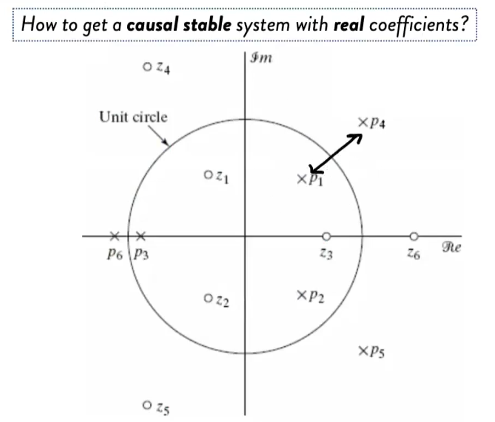
\includegraphics[width=0.6\textwidth]{images/magnitued_square.png}
\end{center}
Given a magnitude response requirement $M(z)$ for $H(z)$, given stability and causality requirements for $H(z)$:
\begin{itemize}
    \item The poles of $H(z)$ are those of $M(z)$ inside the unit circle anda re uniquely identified (for stability constraints)
    \item The zeros of $H(z)$ are not uniquely identified (as zeros influence only the phase and we have no constraints on phase), so the zeros can be both inside and outside the unit circle
    \item Given a causal FIR filter $H(z)$ of order $N$, it has the same magnitude  response $M(z)$ of the causal FIR filter:
    $$G(z)=z^{-N}H^*(z^{-1})$$
    Minimum to maximum phase filter and viceversa
\end{itemize}
From the previous example, in order to have causal and stable system we select the following zeros and poles:
\begin{center}
    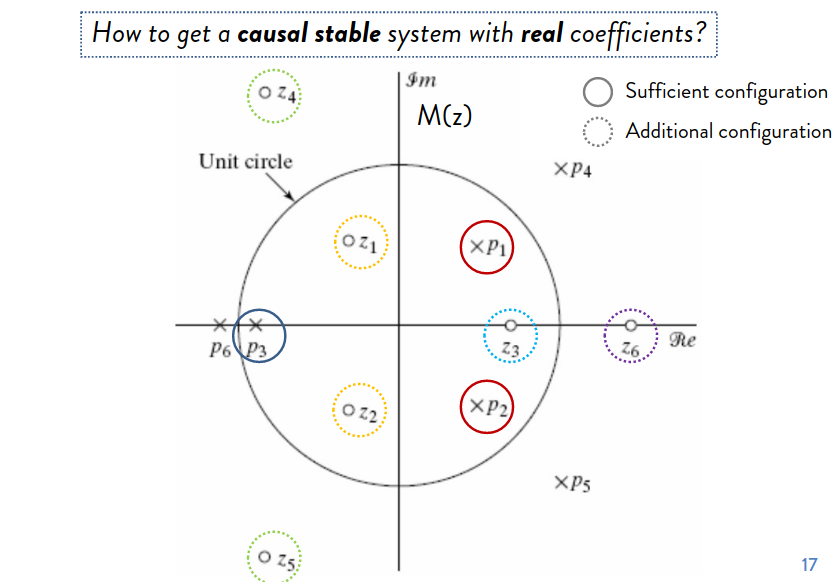
\includegraphics[width=0.6\textwidth]{images/magnitued_square2.png}
\end{center}

\subsubsection{Allpass filters}
Flat behavior in the frequency, which means constant gain and any phase:
$$
|H_{ap}(f)|=|H_{ap}(z)|\big|_{|z|=1}=1\qquad\forall f
$$
Given the previous considerations, a generic causal allpass filter is:
$$
H_{ap}(z)=z^{-K}e^{j\phi}\frac{A(z)}{\tilde{A}(z)}
$$
Where
$$
\begin{cases}
    A(z)=1+a_1z^{-1}+a_2z^{-2}+\cdots+a_Nz^{-N}\\
    \tilde{A}(z)=z^{-N}A^*(z^{-1})=a^*_N+a_{N-1}^*z^{-1}+\cdots+a_2^*z^{2-N}+a_1^*z^{1-N}+z^{-N}
\end{cases}
$$
The denominator is the G version of the numerator, so their magnitudes cancel out.
$$
H_{ap}(z)=z^{-N}e^{j\theta}
\frac{
    1+a_1z^{-1}+a_2z^{-2}+\cdots+a_Nz^{-N}
}{
    a^*_N+a_{N-1}^*z^{-1}+\cdots+a_2^*z^{2-N}+a_1^*z^{1-N}+z^{-N}
}
$$
A general form to represent an allpass real valued impulse response is:
\begin{center}
    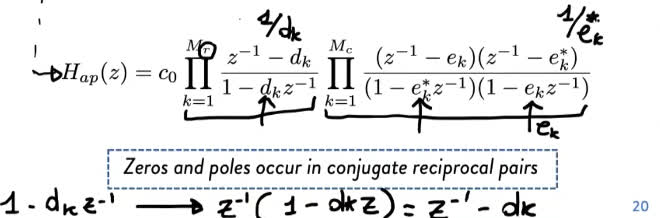
\includegraphics[width=0.6\textwidth]{images/allpass.png}
\end{center}
\textbf{Zeros and poles are in conjugate reciprocal pairs}.
Properties:
\begin{itemize}
    \item Cascade of two allpass filters is again an allpass filter
    \item Each pole of an allpass system is associated with a conjugate reciprocal zero
    \item The magnitude of many cascaded allpass filters is always the same
\end{itemize}